\documentclass[../../Main/Appunti Fisica.tex]{subfiles}
\begin{document}
Si consideri la figura di seguito riportata.
\begin{figure}[!h]
    \centering
    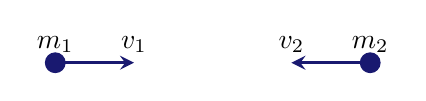
\begin{tikzpicture}[scale = 1, every node/.style={scale=1}]

        % First mass
        \filldraw[MidnightBlue] (0, 0) circle (0.125);
        \node [anchor = south] at (0, 0) {\(m_{1}\)};

        \draw[-stealth, very thick, color = MidnightBlue] (0, 0) -- (1, 0);
        \node [anchor = south] at (1, 0) {\(\va{v_{1}}\)};

        % Second mass
        \filldraw[MidnightBlue] (4, 0) circle (0.125);
        \node [anchor = south] at (4, 0) {\(m_{2}\)};

        \draw[-stealth, very thick, color = MidnightBlue] (4, 0) -- (3, 0);
        \node [anchor = south] at (3, 0) {\(\va{v_{2}}\)};

    \end{tikzpicture}
    \caption{Sistema isolato composto da particelle.}
    \label{fig:7}
\end{figure}
Poiché isolato l'unica forza agente su ciascuna delle due particelle, è quella dovuta all'altra particella.
Segue dunque dalla terza legge di Newton
\[
    \vb{F_{1, 2}} = -\vb{F_{2, 1}} \implies \vb{F_{1, 2}} + \vb{F_{2, 1}} = 0
\]
applicando ora la seconda legge di Newton
\[
    m_{1}\va{a_{1}} + m_{2}\va{a_{2}} = 0
\]
ma da cio, se \(m_{1}, m_{2}\) sono costanti, segue
\[\begin{gathered}
        \dv{(m_{1}\va{a_{1}})}{t} + \dv{(m_{1}\va{a_{2}})}{t} = 0 \\
        \dv{}{t}{(m_{1}\va{a_{1}} + m_{2}\va{a_{2}})} = 0
    \end{gathered}\]
da cui si determina \(m_{1}\va{a_{1}} + m_{2}\va{a_{2}}\) costante.

\begin{Definition*}
    La quantità di moto di un corpo, schematizzabile come punto materiale, di massa \(m\) e velocità \(\vb{v}\), è definita come
    \[
        \va{p} \equiv m\va{v}
    \]
\end{Definition*}
Dall'applicazione della seconda legge di Newton, si possono relazionare forza risultante e quantità di moto, come Segue
\[\begin{aligned}
        \sum \vb{F} & = m\va{a}                            \\
                    & = \dv{(m\va{a})}{t} = \dv{\va{p}}{t}
    \end{aligned}\]

Dunque poiché \(\vb{F_{1, 2}} + \vb{F_{2, 1}} = \dv{}{t}(\va{p_{1}} + \va{p_[2]}) = 0\), segue che \(\va{p_{1}} + \va{p_[2]}\) sia costante.
\begin{Principle*}[di conservazione della quantità di moto]
    Quando due o più corpi di un sistema isolato, interagiscono, la quantità di moto si conserva.
\end{Principle*}
\end{document}